\subparagraph*{Submission : }
\textit{Consider the general case in which the shop needs to optimize the prices and the assignment of promos to the customers in the case all the parameters need to be learnt.}\\

The problem requires to find the optimal prices for the two items and to optimize the assignment of the promos, in the scenario where all the parameters need to be learnt.

\subsection*{Strategy}
We simulate the random arrival of the customers. For every customer we retrieve a superarm from the Thompson sampling learner. A superarm is associated to the couple of the candidates prices of the two items. We evaluate the purchase of the first item at the suggested price. In case the customer buys the first item, we pull the matching from the UCB learner, and we do the same procedure of purchase for the second item at the proposal discounted price. Before the arrival of a new customer, we update the TS learner with the entire reward given by the two items, and the UCB learner with the reward of the second item. We have used the same two matrixes in the same way of the previous request.

\subparagraph{Implementation} 
\subparagraph{Optimal strategy}

\subsection*{Results}
\begin{center}
	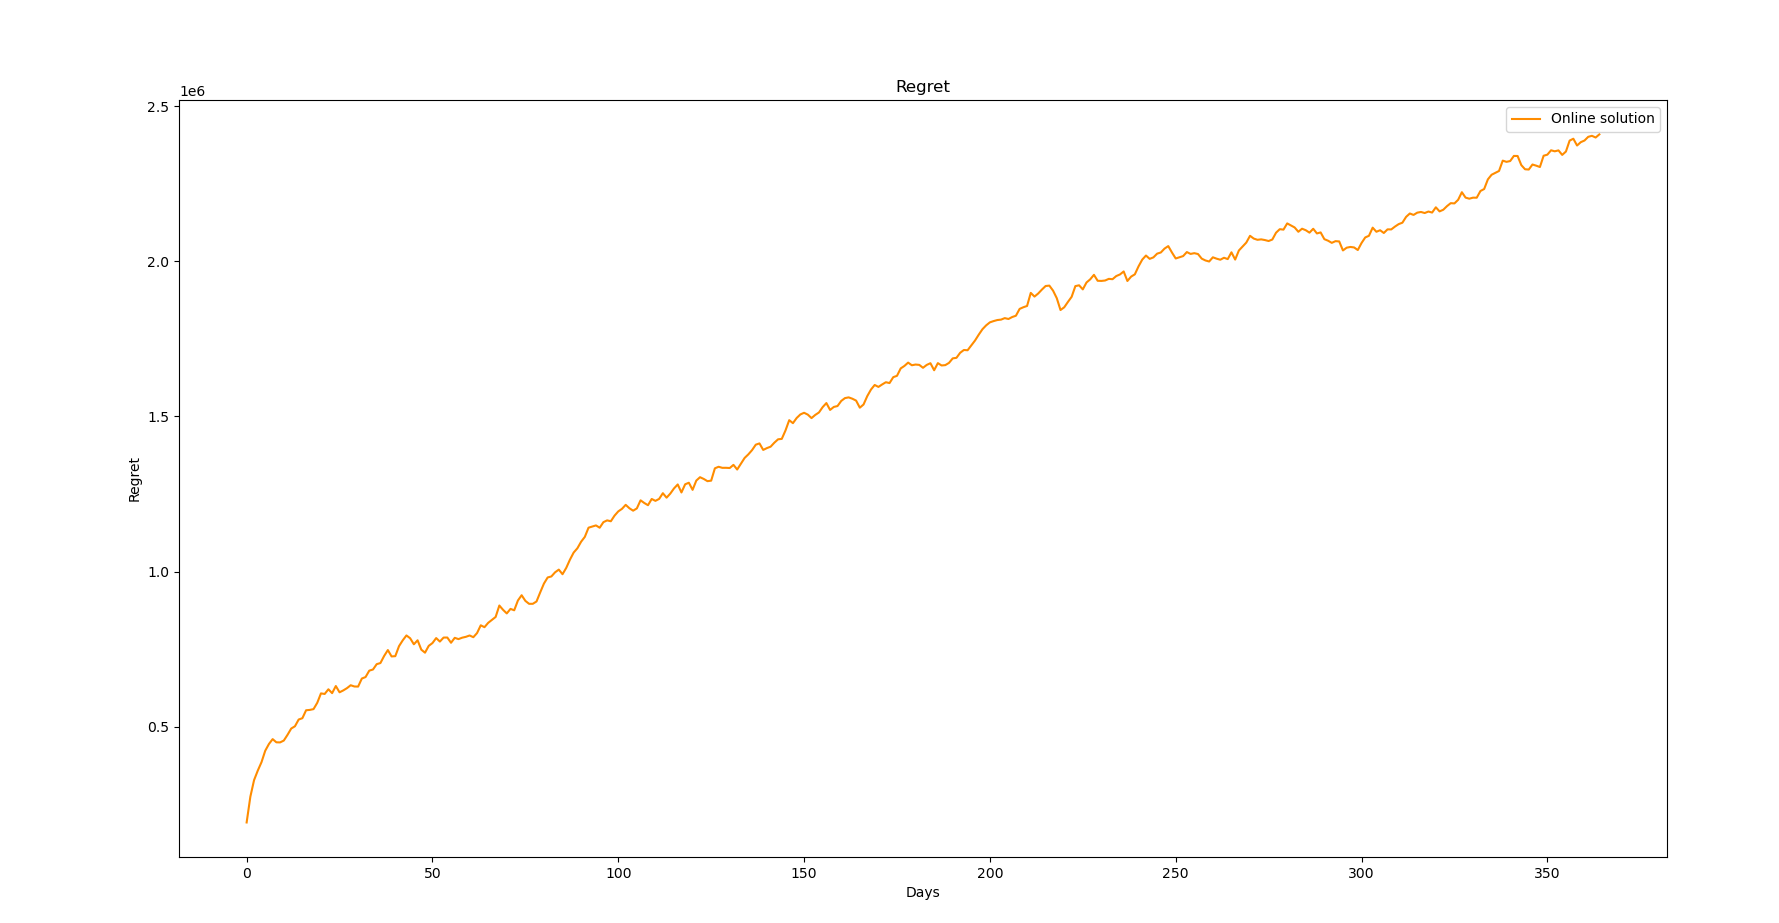
\includegraphics[scale=0.35]{Images/n6}
\end{center}

\subsection*{Considerations}
We can notice that the learners take more time to learn the optimal solutions both for pricing and matching. The cumulative regret is increasing quite linearly until the day 200th, after that, they start to stabilize on the optimal solutions. The cumulative regret still be jagged, because both the learner can pull random arms with some probabilty, this has impact on the curve.